% Author: Izaak Neutelings (September 2020)
\documentclass[border=3pt,tikz]{standalone}
\usepackage{amsmath}
\usepackage{tikz}
\usepackage{physics}
\usepackage{siunitx}
\usepackage[outline]{contour} % glow around text
\usetikzlibrary{angles,quotes} % for pic
\usetikzlibrary{calc}
\contourlength{1.3pt}

\tikzset{>=latex} % for LaTeX arrow head
\usepackage{xcolor}
\colorlet{veccol}{green!70!black}
\colorlet{pathcol}{blue!40!black}
\colorlet{xcol}{blue!70!black}
\colorlet{vcol}{green!70!black}
\colorlet{acol}{red!50!blue!80!black!80}
\colorlet{omcol}{vcol!60!black}
\colorlet{myblue}{blue!70!black}
\colorlet{myred}{red!70!black}
\tikzstyle{vector}=[->,very thick,xcol,line cap=round]
\tikzstyle{mydashed}=[dash pattern=on 2pt off 2pt]
\tikzstyle{mass}=[line width=0.6,red!30!black,fill=red!40!black!10,rounded corners=1,
                  top color=red!40!black!20,bottom color=red!40!black!10,shading angle=20]
\newcommand\rightAngle[4]{
  \pgfmathanglebetweenpoints{\pgfpointanchor{#2}{center}}{\pgfpointanchor{#3}{center}}
  \coordinate (tmpRA) at ($(#2)+(\pgfmathresult+45:#4)$);
  \draw[white,line width=0.6] ($(#2)!(tmpRA)!(#1)$) -- (tmpRA) -- ($(#2)!(tmpRA)!(#3)$);
  \draw[] ($(#2)!(tmpRA)!(#1)$) -- (tmpRA) -- ($(#2)!(tmpRA)!(#3)$);
}


\begin{document}


% CENTRIPETAL ACCELERATION
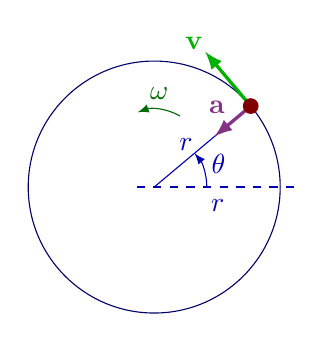
\begin{tikzpicture}
    \def\R{1.6}
    \def\ang{40}
    \coordinate (O) at (0,0);
    \coordinate (X) at (\R,0);
    \coordinate (R) at (\ang:\R);
    \node[inner sep=2] (R') at (R) {};
    \draw[pathcol] (O) circle (\R); %dashed
    \draw[xcol] (O) -- (R) node[midway,below=5,above left=0] {$r$};
    \draw pic[->,"$\theta$",xcol,draw=xcol,angle radius=19,angle eccentricity=1.3] {angle=X--O--R};
    \draw[xcol,dashed] (-0.14*\R,0) -- (1.15*\R,0) node[midway,below=1] {$r$};
    \draw[vector,vcol]
    (R) --++ (\ang+90:0.9) node[above left=-3] {$\vb{v}$};
    \draw[vector,acol]
    (R) --++ (\ang+180:0.6) node[midway,below=0,above left=-1] {$\vb{a}$};
    \fill[red!50!black] (R) circle (0.1);
    \draw[->,omcol] (\ang+30:0.6*\R) arc(\ang+20:\ang+70:0.4*\R) node[midway,above] {$\omega$};
\end{tikzpicture}

\end{document}